\documentclass{article}

\usepackage{amsmath}
\usepackage{hyperref}
\usepackage{graphicx}
\usepackage{booktabs}
\usepackage{amsfonts}
\usepackage{tcolorbox}
\usepackage{amsthm}
\usepackage{listings}
\usepackage{float}
\usepackage{cleveref}
\usepackage{fvextra}
\usepackage[a4paper, margin=1.2in]{geometry}
\usepackage{upgreek}
\usepackage[backend=biber,style=authoryear]{biblatex}
\addbibresource{References.bib}



\graphicspath{ {./images/} }

\title{Reflections on Option Pricing Models}
\author{Tom Beaugé}
\date{January 27, 2025}

\tcbset{
    note/.style={
        colback=black!5,        % Background color
        colframe=black!75, % Frame color
        fonttitle=\bfseries,
        title=Note,
        arc=4mm,               % Rounded corners
        boxrule=1pt,           % Thickness of box frame
        left=6pt,
        right=6pt,
        top=6pt,
        bottom=6pt,
    }
}

\DeclareCiteCommand{\citeauthorlinked}
  {\boolfalse{citetracker} \boolfalse{pagetracker}}
  \printtext{\href{\biburl}{\printnames{labelname}}}
  {\multicitedelim}
  {}



\DefineVerbatimEnvironment{verbatim}{Verbatim}{breaklines=true}

\begin{document}

    \maketitle

    \begin{abstract}
        This document reflects on my self-directed exploration of financial models for option pricing. Being completely new to the world of quantitative finance, I begin with the very basics. In no shape or form is it meant to serve as a reference for others, but rather as a personal log of my progress and understanding of the topic. This means that the document will be filled with personal notes, thoughts, and questions that arise throughout my journey, as well as possible mistakes, misconceptions, and sloppy notation.
        
        \medskip

        Having started this project in the middle of my first year of university, I still lack much of the mathematical background and experience—both in LaTeX and in academic writing in general—that would allow me to make this document as succinct and organized as I would like it to be. Nonetheless, I choose to make all the code public and hope that the reader will notice a gradual improvement in its quality as my journey progresses.
    \end{abstract}

    \section{Introduction}
    \label{sec:introduction}

    The pricing of financial derivatives represents a cornerstone of modern quantitative finance. My project begins with the simplest discrete-time model---the binomial tree---to build intuition about no-arbitrage pricing, risk-neutral valuation, and dynamic hedging. Though elementary, this model encodes key principles that generalize to continuous-time frameworks like the Black-Scholes-Merton model. My goal is to iteratively implement and analyze increasingly sophisticated models, using each step to deepen my understanding of stochastic processes, measure theory, and computational finance.

    Most of the theory gained in this exploration comes from what I will refer to as 'the book', ie. \citetitle{Wilmott2006} by \citeauthor{Wilmott2006}.

    \section{The Binomial Tree Model}
    \label{sec:binomial}

    With its very straightforward concept and basic mathematics, the binomial model seemed like a logical introduction to options pricing. However, this overtly simplistic binary idea that the price of an option can either go up or down is something to be noted. In the words of Paul Wilmott: "the model is for demonstration purposes only, it is not the real thing. As a model of the financial world it is too simplistic, as a concept for pricing it lacks the elegance that makes other methods preferable, and as a numerical scheme it is prehistoric. Use once and then throw away." This word of caution was kept in mind while I sought to implement it based on Chapter 15 of his book \textit{Paul Wilmott Introduces Quantitative Finance}.

    \subsection{A Simple, One-step Binomial Tree}

    In essence, the binomial model, introduced by Cox, Ross, and Rubinstein (1979), provides a discrete-time approximation of asset price dynamics, such that the underlying asset price \( S_t \) evolves in a probability space as:

    \[
        S_{t+1} =
        \begin{cases}
            S_t \cdot u & \text{with probability } p, \\
            S_t \cdot d & \text{with probability } 1 - p.
        \end{cases}
    \]

    where \( u > 1 + r > d > 0 \) ensures arbitrage-free dynamics, and \( r \) is the risk-free rate. Its simplicity belies its ability to replicate derivative payoffs through a self-financing portfolio of the underlying asset and risk-free bonds.

    \subsubsection{Implementation}

    From what was understood, the main idea of the binomial model is to create a risk-neutral valuation. This was achieved by constructing a portfolio composed of the underlying asset and risk-free bonds to exactly match the option's payoff. To prevent any arbitrage, the option's price must thus correspond to the cost of replicating this portfolio. The methodology for constructing this risk-free portfolio was directly inspired by \cite{binomial_options_pricing_yt}, with the slight addition of fixed interest rates to account for the time value of money.

    \medskip

    The relationship governing the replicating portfolio is expressed as:

    \begin{equation}
        \label{eq:delta_hedging_portfolio}
        P_t = \Delta S_t - V_t
    \end{equation}

    Here, \( P_t \) represents the value of the portfolio at time \( t \), \( \Delta \) is the hedge ratio indicating the number of units of the underlying asset held, \( S_t \) is the current price of the underlying asset, and \( V_t \) is the current price of the option. This construction ensures that the portfolio is risk-free by balancing the position in the underlying asset with the short position in the option.

    \medskip

    For the portfolio \( P_t \) to be risk-free, its future value must be identical in both the up and down states. This condition leads to:

    \[
        \Delta S_u - V_u = \Delta S_d - V_d
    \]

    Solving for the hedging ratio \( \Delta \) associated with the number of units of the underlying asset yields:

    \begin{equation}
        \label{eq:delta}
        \Delta = \frac{V_u - V_d}{S_u - S_d}
    \end{equation}

    This calculation ensures that the portfolio replicates the option's payoff in both possible future states, thereby enforcing the no-arbitrage condition.

    \subsubsection{Insights}

    By pricing the option in such a way, we are hedged against any possible fluctuation in price, as the arbitrary probability \emph{p} that the option will increase in price appears at no point in our pricing calculations.
    Playing around with the expected value, I was also able to notice that for a specific probability \emph{p}, the expected value matched the pricing of my option echoing the First Fundamental Theorem of Asset Pricing applies here.

    \begin{tcolorbox}[note, title=First Fundamental Theorem of Asset Pricing]
        The \textbf{First Fundamental Theorem of Asset Pricing} states that a financial market is \textbf{arbitrage-free} if and only if there exists at least one \textbf{equivalent martingale measure} (also known as a risk-neutral measure).

        In other words, the absence of arbitrage opportunities in a market is equivalent to the existence of a probability measure under which discounted asset prices follow a martingale process.
    \end{tcolorbox}

    \bigskip

    \subsubsection*{Deriving the risk neutral probability \emph{p}:}

    Assume the expected return equals the risk-free rate of the underlying asset:

    \[
        \mathbb{E}[S_{t+1}] = (1 + r) S_0
    \]


    where:

    \[
        \mathbb{E}[S_{t+1}] = p S_u + (1 - p) S_d
    \]

    Thus, solving for the risk-neutral probability \(p\) yields:

    \begin{equation}
        \label{eq:risk_neutral_prob_discrete}
        p = \frac{1 + r - d}{u - d}
    \end{equation}

    \subsubsection{Limits}

    Its assumptions---constant \( u \), \( d \), \( r \), and no transaction costs---are economically restrictive.
    Moreover, the model oversimplifies price fluctuations to just an up and down movement.
    It's also completly inadapted for more complex options, very poorly estimates those with longer expirations and does not account for volatility.

    \medskip

    These limitations motivate the need for more sophisticated models.

    \subsubsection{Future Directions}

    This work lays the groundwork for several extensions:

    \begin{itemize}
        \item \textbf{Multi-Period Trees}: Generalizing to \( n \)-period trees to approximate continuous processes.
        \item \textbf{American Options}: Incorporating early exercise features via dynamic programming.
        \item \textbf{Volatility}: Experimenting with time-varying \( u \) and \( d \) to model volatility.
    \end{itemize}


    \subsection{Going Multi-step}

    The next step in my exploration was to extend the single-step binomial tree to a multi-period framework.
    This extension allows for a improvements in the modelisation of our asset price, allowing us to have a rudimentary estimate of the option's price over a larger period of time.
    The fluctuations in the asset price are still binary, but this new improvement allow us to better represent the random walk of our asset.

    \subsubsection{Implementation}

    To simplify the calculations, I have decided to only carry the theory from our previous one-step model.
    Our simple one-period option was priced using the hedge ratio \(\Delta\).
    However, to make the computation more straightforward, I have chosen to reuse the risk-neutral probability \(p\) we found earlier to price the option at each node.

    \begin{enumerate}

        \item \textbf{Building the Stock Price Tree:} A two-dimensional array is used to store the possible stock prices at maturity. At each node corresponding to \( i \) upward movements (and \( n-i \) downward movements) after \( n \) steps, the stock price is calculated as:
        \[
        S_{n,i} = S_0 \, u^i \, d^{n-i},
        \]
        where \( S_0 \) is the initial stock price.

        \item \textbf{Option Payoff Calculation:} At maturity, the option payoff is computed at each node. For a call option, the payoff is:
        \[
        \text{Payoff} = \max(S_{n,i} - K, 0),
        \]
        and for a put option:
        \[
        \text{Payoff} = \max(K - S_{n,i}, 0),
        \]
        where \( K \) is the strike price.

        \item \textbf{Backward Induction:} After setting the terminal payoffs, the tree is traversed backward to compute the option value at earlier nodes. At each node, the option value is obtained as:
        \[
        V_{i,j} = \frac{p \, V_{\text{up}} + (1 - p) \, V_{\text{down}}}{1 + r},
        \]
        where:
        \begin{itemize}
            \item \( V_{\text{up}} \) is the option value from the node corresponding to an upward movement,
            \item \( V_{\text{down}} \) is the option value from the node corresponding to a downward movement,
            \item \( 1 + r \) is used to incorporate the risk-free rate per period.
        \end{itemize}
        This backward induction continues until the root node is reached, where the option price at time zero is obtained.
    \end{enumerate}


    A short code excerpt is shown below:

    \small
    \begin{verbatim}
    public MultiStepBinomialTree(double initialPrice, double strikePrice,
            double probabilityUp, double upFactor, double downFactor,
            double interestRate, boolean isCall, int steps) {

        // Calculating risk-neutral probability: q = (1 + r - d) / (u - d)
        double q = calculateRiskNeutralProbability(upFactor, downFactor, interestRate);

        // Initializing arrays for stock prices and option values
        stockPriceMaturity = new double[steps + 1][steps + 1];
        optionValues = new double[steps + 1][steps + 1];

        // Backward induction to build the tree and calculate option values
        for (int step = steps; step >= 0; step--) {
            for (int i = 0; i <= step; i++) {
                // Calculate stock price at the node: S = initialPrice * u^i * d^(step-i)
                stockPriceMaturity[step][i] = initialPrice * Math.pow(upFactor, i) * Math.pow(downFactor, step - i);

                // Set option payoff at maturity or compute the option value by backward induction
                if (step == steps) {
                    optionValues[step][i] = calculateOptionPayoff(stockPriceMaturity[step][i], strikePrice, isCall);
                } else {
                    optionValues[step][i] = calculateOptionValue(optionValues[step + 1][i], optionValues[step + 1][i + 1], interestRate, q);
                }
            }
        }
    }
    \end{verbatim}

    \normalsize

    \emph{Note:} The code snippet is a simplified version of the actual implementation, which includes additional error handling and input validation.

    \medbreak

    The final option price is available as the value of the root node of the tree, i.e., \texttt{optionValues[0][0]}. This represents the present value of the option under the given parameters and assumptions of the binomial model.

    \medbreak

    \textbf{Example Case}
    To illustrate the implementation, consider the following example:

    \begin{itemize}
        \item Initial stock price (\( S_0 \)): \$100
        \item Strike price (\( K \)): \$105
        \item Up factor (\( u \)): 1.1
        \item Down factor (\( d \)): 0.9
        \item Risk-free rate (\( r \)): 5\% per period
        \item Number of steps: 3
        \item Option type: Put
    \end{itemize}

    \begin{figure}[H]
        \centering
        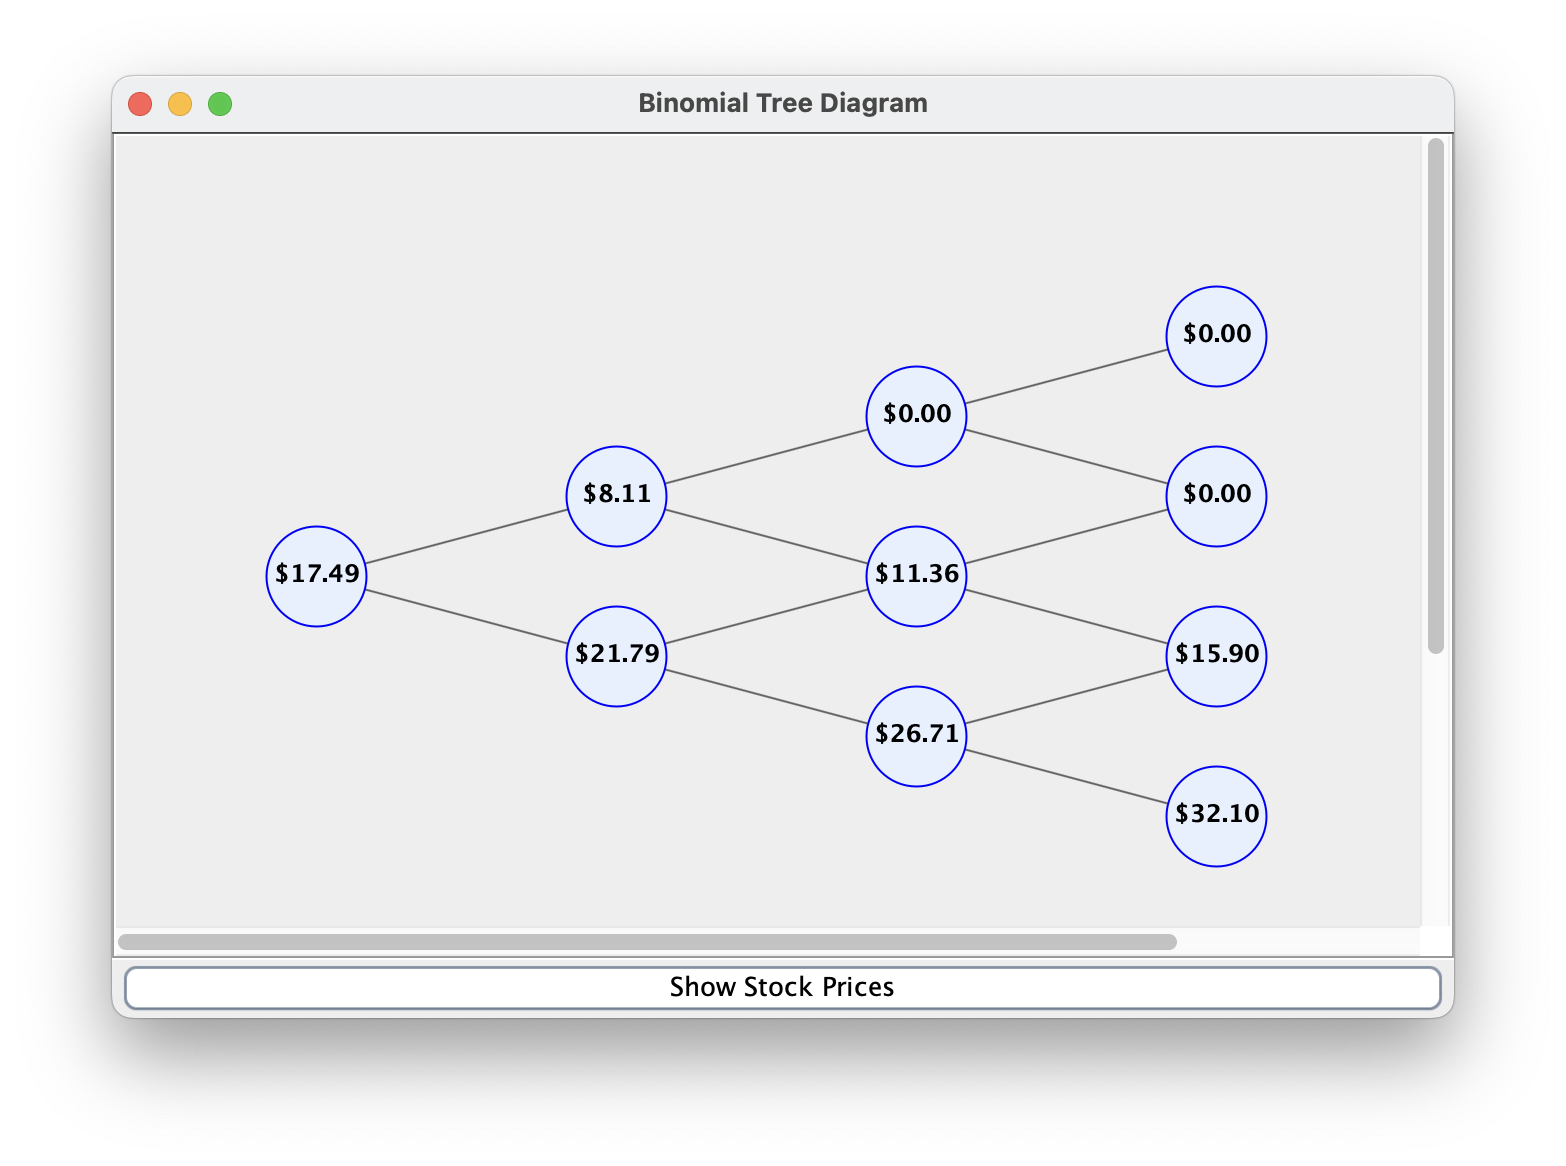
\includegraphics[scale=0.4]{Example1_BinTree_OptionValue}
        \caption{Option values for a 3-step tree}
        \label{fig:3_step_option_tree}
    \end{figure}

    \begin{figure}[H]
        \centering
        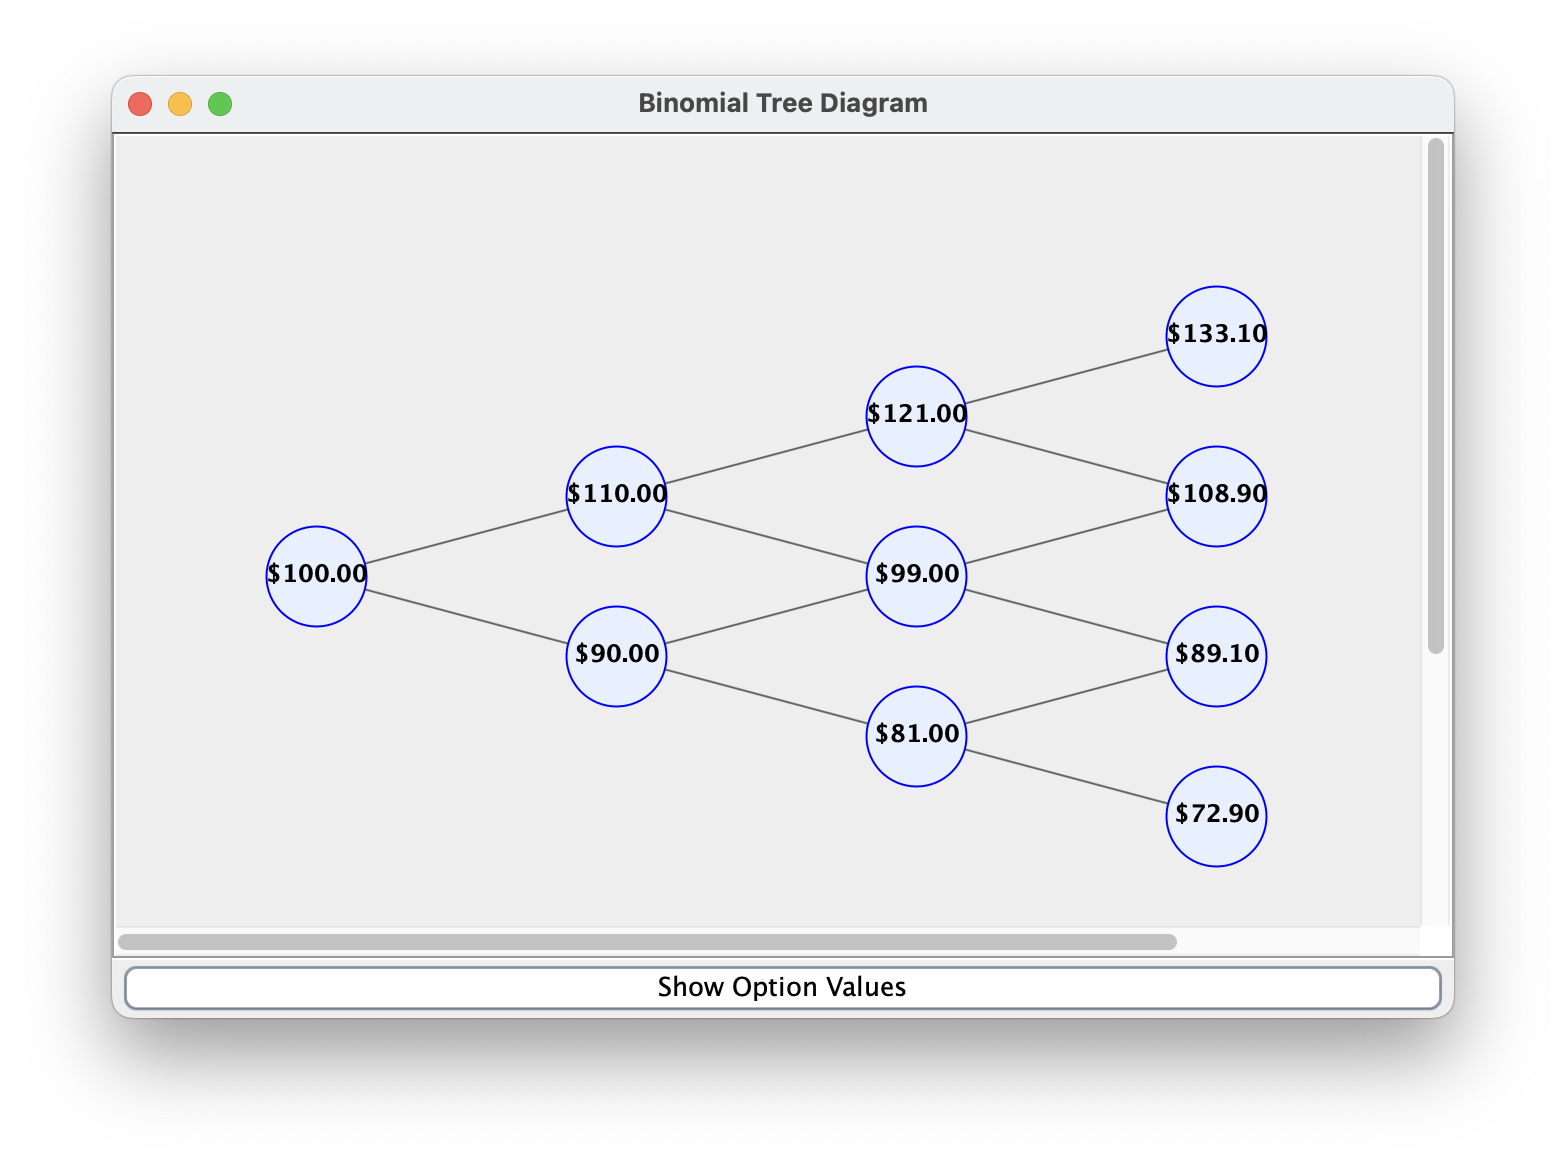
\includegraphics[scale=0.4]{Example1_BinTree_StockPrice}
        \caption{Stock prices}
        \label{fig:3_step_stock_price_tree}
    \end{figure}

    The rightmost nodes in Figure~\ref{fig:3_step_option_tree} show the payoffs of the put option at expiration, computed as:
    \[
    P_T = \max(K - S_T, 0)
    \]
    Some nodes have a value of \$0.00, indicating that the stock price was above the strike price at expiration, making the put option worthless.

    \medskip

    The deeper the stock price falls below \( K = 105 \), the higher the put option value. The highest option price is observed in paths where the stock price significantly declines.

    The root node of the tree gives an option price of \$17.49, which represents the fair value of the put option under these assumptions.

    \subsubsection{Insights}


    The following figure illustrates the evolution of computation time as the number of steps increases in the multi-step binomial tree model.

    \begin{figure}[h]
        \centering
        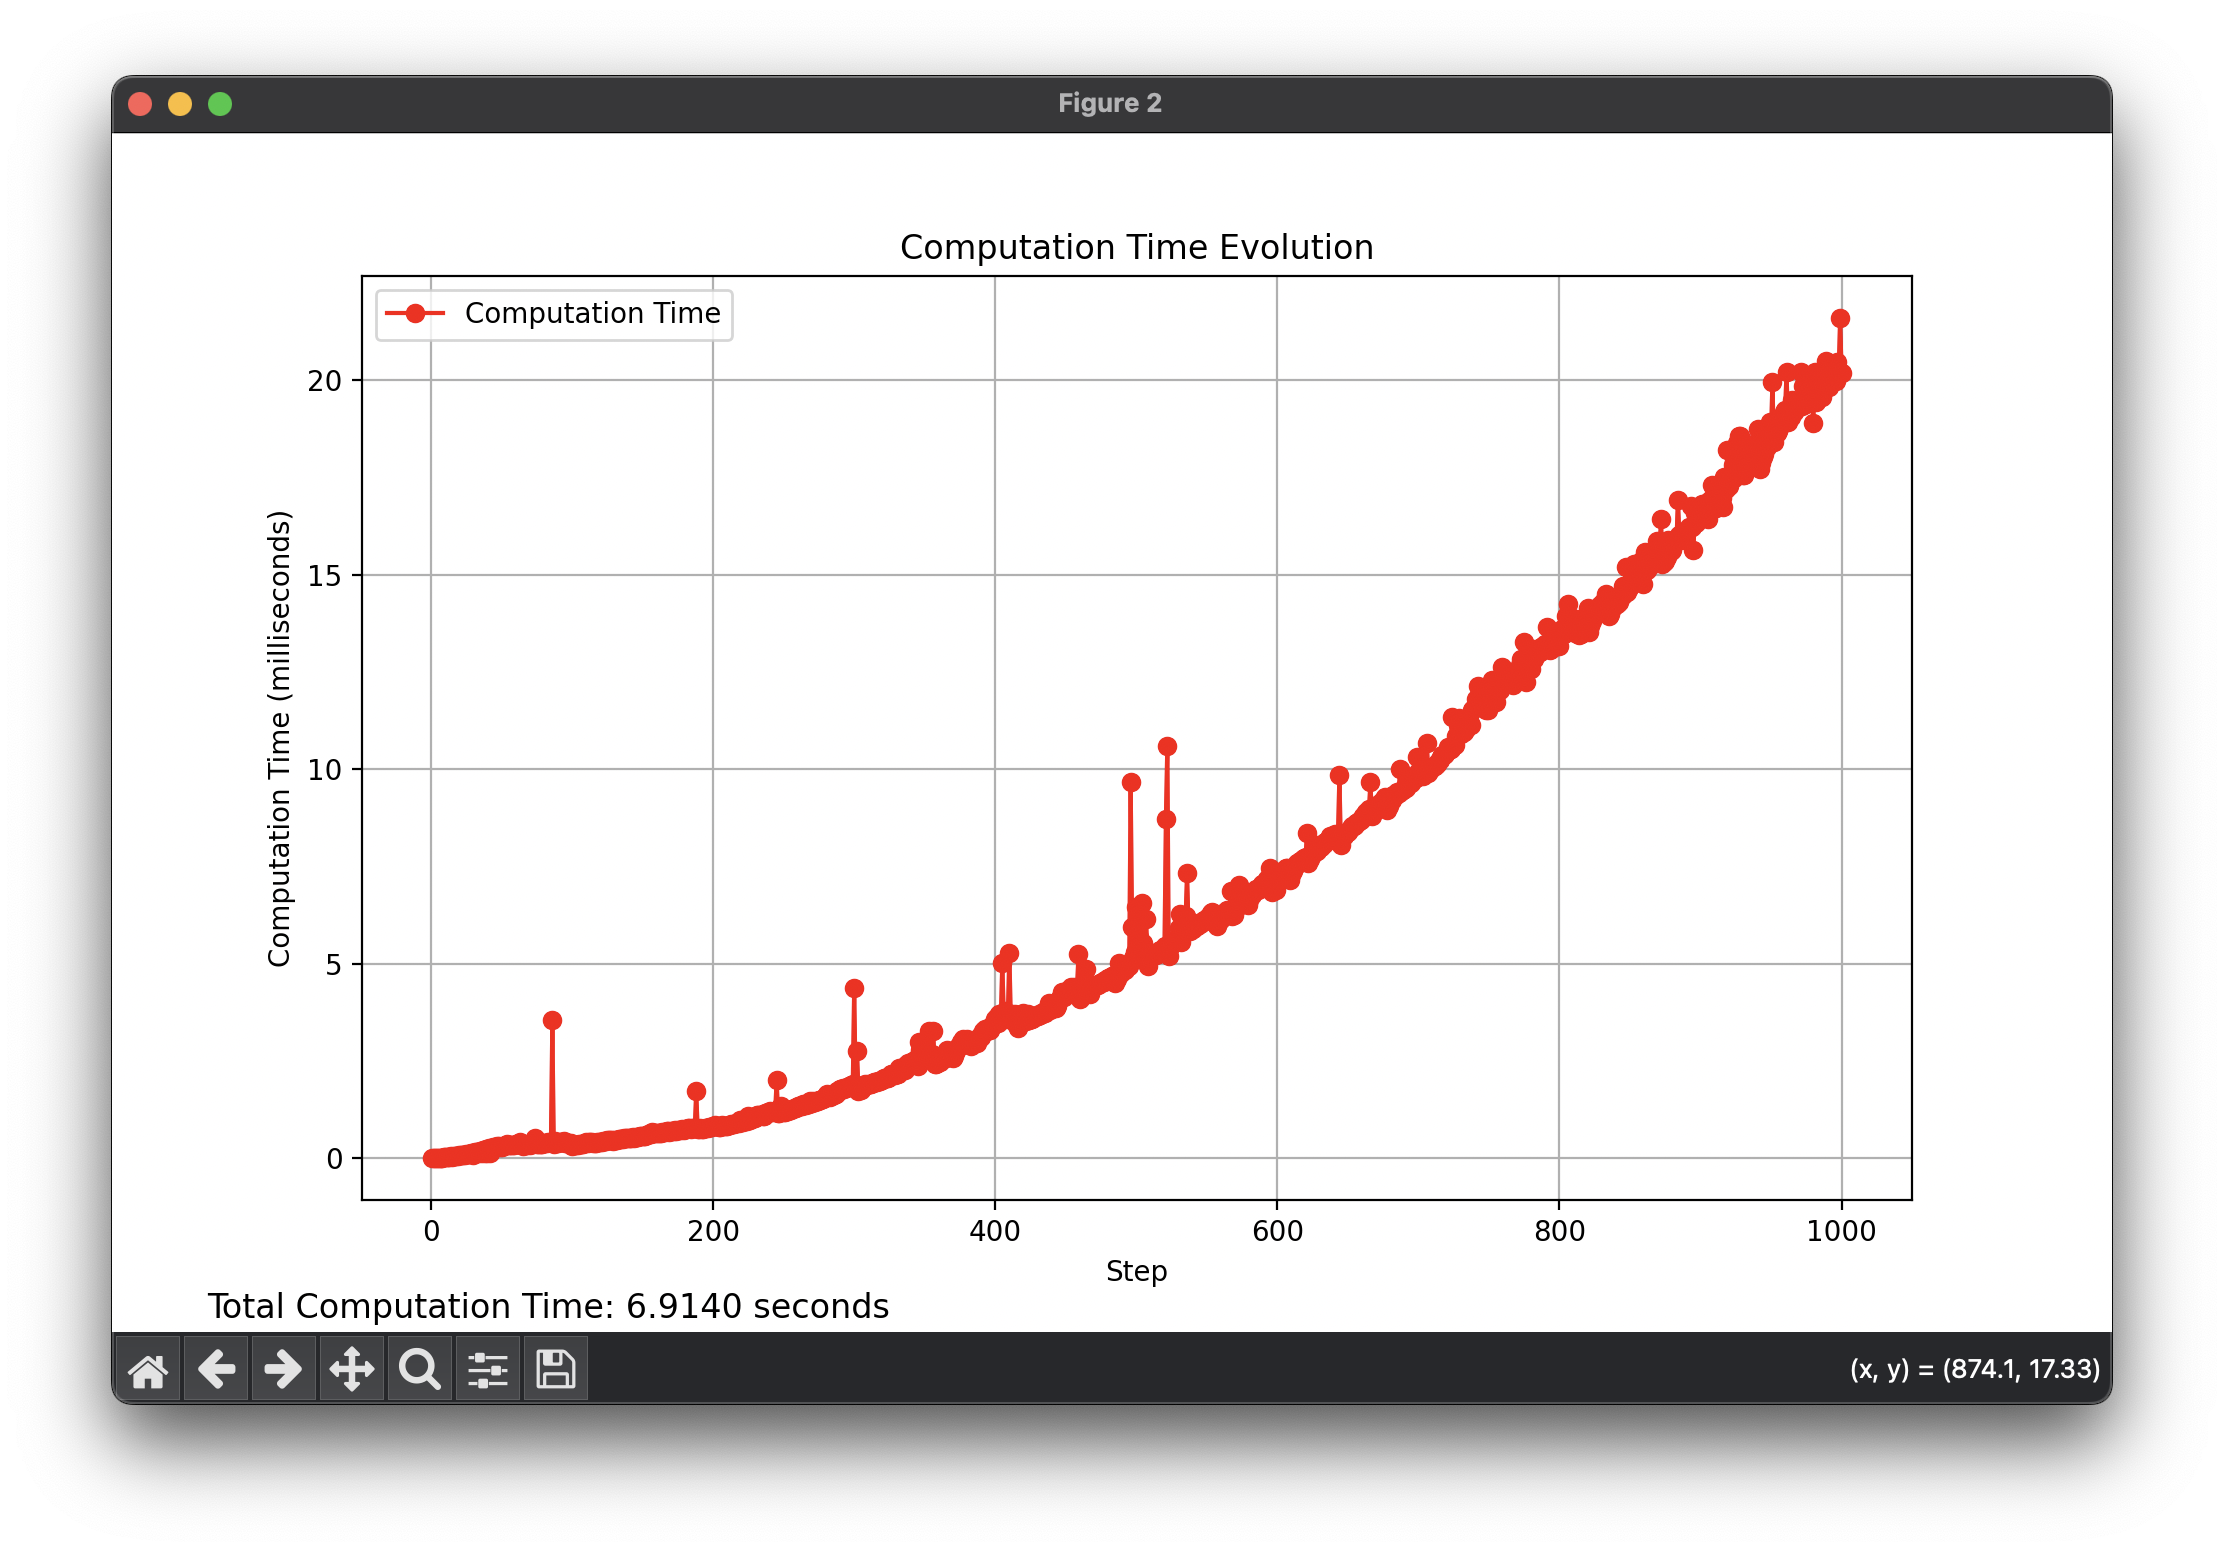
\includegraphics[width=0.8\textwidth]{ComputationTime_BinTree_v1}
        \caption{Computation time for Binomial Trees up to 1000 steps)}
        \label{fig:computation_time_bintree_v1}
    \end{figure}

    The observed quadratic trend in computation time suggests that the model’s complexity scales poorly with large steps. Optimization strategies such as dynamic programming, parallel processing, and memory-efficient algorithms should be explored to improve performance.
    If we look at the code snippet above, the time complexity is dominated by the nested loops:

    \bigbreak

    Outer loop: Iterates over steps from \( n \) to \( 0 \) (total \( n + 1 \) steps).
    Inner loop: For each step \( s \), iterates \( i \) from \( 0 \) to \( s \) (total \( s + 1 \) iterations per step).

    \medbreak
    Per-node operations:

    For each node \( ( \text{step}, i ) \), \texttt{calculateOptionValue} computes the option value using:

    \[
        \text{Value} = \frac{q \cdot \text{Payoff}_{\text{Up}} + (1 - q) \cdot \text{Payoff}_{\text{Down}}}{1 + r}
    \]

    Nonetheless, while most operations to calculate the payoff is constant time (\emph{see code above}), \emph{Math.pow} is of complexity \( O(\log n) \).

    \bigskip

    This simplifies to a total time complexity of:
    \[
    O(n^2 \log n)
    \]

    \bigbreak

    \emph{note that the graphs rather represent a \( O(n^3 \log n) \) complexity as they plot binomials tree from 1 to n-steps}

    \bigbreak

    As a general benchmark, the current implementation computes in 10 seconds binomial trees up to 1100 steps with the memory usage that maxes out around 225MB.
    The current challenge is to enhance computational speed while simultaneously optimizing memory efficiency.

    \subsubsection{Speeding up the process}

    Given the quadratic growth in computation time and the substantial memory footprint, several optimizations were implemented to enhance both speed and memory efficiency in the multi-step binomial tree model.

    \paragraph{1. Precomputing Powers}
    Repeated calls to \texttt{Math.pow} were identified as a significant performance bottleneck, given their logarithmic time complexity \(O(\log n)\).
    To address this the increase and decrease factors are now precomputed using induction:

    \begin{verbatim}
        double[] upPowers = new double[steps + 1];
        double[] downPowers = new double[steps + 1];
        upPowers[0] = 1.0;
        downPowers[0] = 1.0;
        for (int j = 1; j <= steps; j++) {
            upPowers[j] = upPowers[j - 1] * upFactor;
            downPowers[j] = downPowers[j - 1] * downFactor;
        }
    \end{verbatim}

    This optimization reduces the total time complexity from:

    \[
        O(n^2 \log n) \quad \text{to} \quad O(n^2)
    \]

    This results in a major time-related improvement - 2800 steps are now computed in 10 seconds - but now significantly more memory is used, peaking around 1600MB.

    \paragraph{2. Allocating jagged arrays}
    Instead of assigning a square array for our stock price and option value through time, leading to unnecessary empty entries, each row was allocated with the exact size they needed (i.e.\ step number + 1)


    This led to some improvements in the memory usage which now maxes around 1300MB. Its time efficiency also increased reaching 3100 steps in 10 seconds.
    This is hypothesized to be due to a reduction in garbage collection pressure as well as a better cache utilisation since no superfluous data is present.

    \paragraph{Summary}

    With the implementation of storing stock and option values for every node, the code has been optimised.
    Parallelising computations was deemed unnecessary, as most operations depend on previous inputs. While its implementation led to noticeable improvements, it was perhaps even counterproductive for smaller step sizes.
    It could nonetheless be used to speed up the process of computing all binomial trees for our graphs since they are calculated independently but as of right now we have enough data points.
    The focus should remain on establishing a valid and efficient model.

    \medskip

    Further optimisations would likely require better hardware configurations (which are beyond the scope of this project) or the adoption of a language with more efficient memory management, such as Rust, or a more 'hands-on' language like C++.

    \medskip

    Overall, the performance upgrade is significant. Previously, computing trees up to 1000 steps took over 6 seconds, whereas the optimised program now completes the same task in under half a second. This improvement enables data extraction after a large number of steps, better reflecting the constant fluctuations of real-world assets. However, the \( O(n^2) \) time complexity still limits the model's long-term usability, highlighting the need for a more efficient model in this regard.

    \subsection{Towards continuity}

    We now aim to transition from our discrete model to a continuous framework, while retaining much of the underlying theory.
    Consequently, the option price can still be expressed using the familiar formula:

    \begin{equation}
        \label{eq:option_price}
        V = \frac{p \, V_{\text{up}} + (1 - p) \, V_{\text{down}}}{1 + r \updelta t},
    \end{equation}

    Notice the subtle yet important modification: we've replaced $1 + r$, the discrete discount factor, with $1 + r \updelta t$, which approximates the continuous compounding factor $e^{1 + r \updelta t}$.
    This adjustment bridges the gap between discrete and continuous discounting, setting the stage for a smooth transition to continuous-time option pricing models.

    We will now assume that our underlying asset follows a Geometric Brownian Motion (GBM).
    While this choice is primarily guided by the model used in the reference book, its advantages are evident.

    It captures randomness in a mathematically straightforward manner, which will help us greatly in the calculations to come.
    Additionally, its logarithmic nature ensures that the asset price remains strictly positive, which aligns with real-world financial behavior

    However, it’s important to acknowledge a key limitation: while assuming constant volatility simplifies the model and offers analytical convenience, it does not accurately reflect the dynamic nature of volatility observed in real markets.
    This simplification, though useful for theoretical development, should be considered with caution when interpreting real-world applications.

    \subsubsection{Finding the up facor \emph{u} and down factor \emph{d}}

    Our initial assumption that $V_{\text{up}} = u V$ and $V_{\text{down}} = v V$ now proves itself incompatible with Brownian motion.

    Instead, for an asset price $S_t$ that follows GBM, its dynamics are given by the stochastic differential equation:

    \begin{equation}
        \label{eq:gbm}
        dS_t = \mu S_t\, dt + \sigma S_t\, dW_t,
    \end{equation}

    where:
    \begin{itemize}
        \item $\mu$ is the drift
        \item $\sigma$ is the volatility
        \item $W_t$ is the standard Brownian motion
    \end{itemize}

    \bigskip

    \begin{tcolorbox}[note, title=Stochastic Calculus]
        A defining feature of stochastic calculus is its ability to handle processes whose paths are nowhere differentiable, such as Brownian motion.
        Unlike smooth functions in standard calculus, the trajectory of a Brownian motion is highly irregular, exhibiting infinite fluctuations over any time interval, no matter how small.
    \end{tcolorbox}

    \bigskip

    Using a solution of this differential found on Wikipedia we find the following equation:

    \[
        S_{t+\delta t} = S_t \exp
        \bigg\{
        \underbrace{\bigg( \mu - \frac{1}{2} \sigma^2 \bigg) \delta t}_{\text{Deterministic term}}
        +
        \underbrace{\sigma \sqrt{\delta t} \, \epsilon}_{\text{Stochastic term}}
        \bigg\}
    \]

    where $\epsilon$ is the standard normal random variable

    \bigskip

    Since the deterministic term is constant:

    \[E\!\left[\frac{S_{t+\delta t}}{S_t}\right] = e^{\left( \mu - \frac{1}{2} \sigma^2 \right) \delta t} E\!\left[e^{\sigma \sqrt{\delta t} \, \epsilon}\right] \]

    \bigskip

    An interesting formula found in~\cite[p.~637]{Ross2010} can be used here:

    \[E\left[e^{aW}\right] = e^{a E[W] + \frac{1}{2} a^2 \, \text{Var}(W)}\]

    where $W$ is a standard normal random variable.

    \bigskip

    In our case we may consider $W$ to be $\epsilon$, thus $E[W] = 0$ and $\text{Var}(W) = 1$

    It follows that

    \[E\!\left[e^{\sigma \sqrt{\delta t} \, \epsilon}\right] = e^{\frac{1}{2} \sigma^2 \delta t} \]

    Hence

    \begin{equation}
        \label{ev_bintree_dt}
        E\!\left[\frac{S_{t+\delta t}}{S_t}\right] = e^{\left( \mu - \frac{1}{2} \sigma^2 \right) \delta t} e^{\frac{1}{2} \sigma^2 \delta t} = e^{\mu \delta t}
    \end{equation}

    \bigskip

    To find the variance:

    \[\operatorname{Var}\left[\frac{S_{t+\delta t}}{S_t}\right] = E\!\left[\left(\frac{S_{t+\delta t}}{S_t}\right)^2\right] - E\!\left[\frac{S_{t+\delta t}}{S_t}\right]^2\]

    \bigskip

    Fistly,

    \begin{align*}
        E\left[\left(\frac{S_{t+\delta t}}{S_t}\right)^2\right]
        &= \mathbb{E}\!\left[ e^{ 2 \delta t\left( \mu - \frac{1}{2} \sigma^2 \right) + 2 \sigma \sqrt{\delta t} \, \epsilon} \right] \\
        &= e^{2 \delta t\left( \mu - \frac{1}{2} \sigma^2 \right)} \cdot \mathbb{E}\!\left[e^{2 \sigma \sqrt{\delta t} \, \epsilon}\right] \\
        &= e^{2 \delta t\left( \mu - \frac{1}{2} \sigma^2 \right)} \cdot e^{2 \sigma^2 \delta t} \\
        &= e^{2 \mu \delta t + \sigma^2 \delta t}
    \end{align*}

    Secondly,

    \[E\left[\frac{S_{t+\delta t}}{S_t}\right]^2 = e^{2 \mu \delta t}\]

    \bigskip

    \[\implies \operatorname{Var}\left[\frac{S_{t+\delta t}}{S_t}\right] = e^{2 \mu \delta t} (e^{\sigma^2 \delta t} - 1)\]

    Since $\delta t \to 0$, we may use the approximations:

    \begin{align*}
        e^{2 \mu \delta t} &\approx 1 + 2 \mu \delta t \\
        e^{\sigma^2 \delta t} &\approx 1 + \sigma^2 \delta t
    \end{align*}


    \begin{equation}
        \label{var_bintree_dt}
        \implies \operatorname{Var}\!\left[\ln\!\left(\frac{S_{t+\delta t}}{S_t}\right)\right] = \sigma^2\, \delta t
    \end{equation}

    Having established the expected value and variance of \( \frac{S_{t+\delta t}}{S_t} \), we now  construct our two equations in order to approximate the up and down factors, \( u \) and \( d \).

We model the price movement over \( \delta t \) as a binary outcome:

\[
    \frac{S_{t+\delta t}}{S_t} = 
    \begin{cases}
        u, & \text{with probability } p, \\
        d, & \text{with probability } 1 - p.
    \end{cases}
\]

To ensure consistency with the GBM process, we match the first two moments (mean and variance) of this discrete distribution with those derived earlier.

\paragraph{Matching the Expected Value}
From equation~(\ref{ev_bintree_dt}):

\[
    E\!\left[\frac{S_{t+\delta t}}{S_t}\right] = p u + (1 - p) d = 1 + \mu \delta t
\]

where we have used the approximation \( e^{\mu \delta t} \approx 1 + \mu \delta t \) for small \( \delta t \).

\paragraph{Matching the Variance}
From equation~(\ref{var_bintree_dt}):

\[
    \operatorname{Var}\!\left[\frac{S_{t+\delta t}}{S_t}\right] = p u^2 + (1 - p) d^2 - (p u + (1 - p) d)^2 = \sigma^2 \delta t
\]

\paragraph{Symmetric Case (\( p = 0.5 \))}
For simplicity, let us consider a symmetric model where \( p = \frac{1}{2} \). This assumption leads to:

\[
    \frac{u + d}{2} = 1 + \mu \delta t, \quad \frac{u^2 + d^2}{2} - \left(1 + \mu \delta t\right)^2 = \sigma^2 \delta t
\]

Solving the first equation for \( d \):

\[
    d = 2(1 + \mu \delta t) - u
\]

Substituting into the variance equation:

\[
    \frac{u^2 + (2(1 + \mu \delta t) - u)^2}{2} - (1 + \mu \delta t)^2 = \sigma^2 \delta t
\]

Expanding and simplifying under the assumption that \( \delta t \to 0 \), we obtain:

\[
    u = 1 + \sigma \sqrt{\delta t}, \quad d = 1 - \sigma \sqrt{\delta t}
\]

\subsubsection{Finding the Risk-Neutral Probability}

To solve for the risk-neutral probability \( p \), we can directly use the equation ~(\ref{eq:risk_neutral_prob_discrete}) we derived earlier, while accounting for the interest rate \( r \) what we know consider continuous:

\begin{equation}
    \label{eq:risk_neutral_prob_continuous}
    p = \frac{(1 + r \delta t) - d}{u - d}.
\end{equation}

Next, we substitute our approximations for \( u \) and \( d \) into \( p \):

\begin{align*}
    p &= \frac{(1 + r \delta t) - (1 - \sigma \sqrt{\delta t})}{(1 + \sigma \sqrt{\delta t}) - (1 - \sigma \sqrt{\delta t})} \\
    &= \frac{r \delta t + \sigma \sqrt{\delta t}}{2 \sigma \sqrt{\delta t}} \\
    &= \frac{r \delta t}{2 \sigma \sqrt{\delta t}} + \frac{\sigma \sqrt{\delta t}}{2 \sigma \sqrt{\delta t}} \\
    &= \frac{r \sqrt{\delta t}}{2 \sigma} + \frac{1}{2}.
\end{align*}

\bigskip

\noindent
\textbf{Final Expression:}

\begin{equation}
    \label{eq:solved_risk_neutral_prob_continuous}
    \boxed{p = \frac{1}{2} + \frac{r \sqrt{\delta t}}{2 \sigma}}
\end{equation}
    

As \( \delta t \to 0 \), the second term diminishes, and \( p \) approaches \( \frac{1}{2} \). This reflects the symmetric nature of price movements in the continuous-time limit, with a slight adjustment based on the risk-free rate \( r \).

\subsubsection{Applying our delta hedging strategy to a continuous time frame}
\label{sec:deriving_continuous}

Here again we follow the framework we have established with our discrete time binomial model.

We may use the same delta hedging strategy as before, given by ~\ref{eq:delta_hedging_portfolio}:

\[
    \Pi = V(S, t) - \Delta S.
\]

\noindent\textbf{\textit{NB:}} My portfolio $P$ is now denoted $\Pi$ in order to adopt more rigorous notation.


As a reminder, our goal is to eliminate risk by choosing \( \Delta \) such that the portfolio becomes \emph{risk-free} over a small time interval \( \delta t \).

Since the portfolio is risk-free, it must grow at the risk-free rate \( r \). Thus, the change in portfolio value satisfies:

\[
    d\Pi = r \Pi \, dt.
\]


\paragraph{Taylor Expansion for the Option Value}
\label{paragraph:taylor_expansion_option_value}

Consider the option value at the next time step for an upward and downward move:

\[
    V_{up} = V(uS, t + \delta t), \quad V_{down} = V(dS, t + \delta t).
\]

Expanding \( V_{up} \) around \( (S, t) \) using a Taylor series:

\[
    V_{up} \approx V(S, t) + \frac{\partial V}{\partial S}(uS - S) + \frac{\partial V}{\partial t} \delta t + \frac{1}{2} \frac{\partial^2 V}{\partial S^2} (uS - S)^2.
\]

Similarly, for \( V_{down} \):

\[
    V_{down} \approx V(S, t) + \frac{\partial V}{\partial S}(dS - S) + \frac{\partial V}{\partial t} \delta t + \frac{1}{2} \frac{\partial^2 V}{\partial S^2} (dS - S)^2.
\]

Using the approximations,

\[
    u = 1 + \sigma \sqrt{\delta t}, \quad d = 1 - \sigma \sqrt{\delta t},
\]

We find:

\[
    uS - S = \sigma S \sqrt{\delta t}, \quad dS - S = -\sigma S \sqrt{\delta t}.
\]

\paragraph{Constructing our Risk-Free Portfolio}

Since a risk-free portfolio has no randomness, we are only concerned with the expected change in the portfolio over $\delta t$:

 \begin{equation*}
    \label{eq:delta_hedging_change_portfolio}
    d\Pi = dV - \Delta \, dS
 \end{equation*}


 The expected change in the option value is:

 \[
 E[\Delta V] = p(V_{up} - V) + (1 - p)(V_{down} - V)
 \]

 While for our change in the stock value:

 \[
    - \Delta \, dS = -\Delta \left( p(u - 1)S + (1 - p)(d - 1)S \right)
 \]


Combining both changes:

\[
    d\Pi = p (V{up} - V) + (1 - p)(V_{down} - V) - \Delta (p(u - 1)S + (1 - p)(d - 1)S).
\]

Substituting the Taylor expansions:

\begin{align*}
    d\Pi &= p \left( \frac{\partial V}{\partial S} \sigma S \sqrt{\delta t} + \frac{\partial V}{\partial t} \delta t + \frac{1}{2} \frac{\partial^2 V}{\partial S^2} \sigma^2 S^2 \delta t \right) \\
    &+ (1 - p) \left( -\frac{\partial V}{\partial S} \sigma S \sqrt{\delta t} + \frac{\partial V}{\partial t} \delta t + \frac{1}{2} \frac{\partial^2 V}{\partial S^2} \sigma^2 S^2 \delta t \right) \\
    &- \Delta \left( p \sigma S \sqrt{\delta t} - (1 - p) \sigma S \sqrt{\delta t} \right).
\end{align*}

Grouping terms:

\begin{align*}
    d\Pi &= (2p - 1) \sigma S \sqrt{\delta t} \left( \frac{\partial V}{\partial S} - \Delta \right) \\
    &+ \left( \frac{\partial V}{\partial t} + \frac{1}{2} \sigma^2 S^2 \frac{\partial^2 V}{\partial S^2} \right) \delta t.
\end{align*}

Substituting the Taylor expansions and simplifying:

\[
    d\Pi \approx \left( \frac{\partial V}{\partial t} + \frac{1}{2} \sigma^2 S^2 \frac{\partial^2 V}{\partial S^2} \right) \delta t.
\]

Using \ref{eq:delta}:
\begin{align}
    \nonumber
    \Delta &= \frac{V_{up} - V_{down}}{S_{up} - S_{down}} \\
    \nonumber
    &= \frac{2 \frac{\partial V}{\partial S} \sigma S \sqrt{\delta t}}{2 \sigma S \sqrt{\delta t}} \\
    &= \frac{\partial V}{\partial S} \label{eq:risk_neutral_delta}
\end{align}


\paragraph{Applying the No-Arbitrage Condition}

Our portfolio must also satisfy the no-arbitrage condition, meaning it must grow at the risk-free rate $r$. Thus, the change in portfolio value satisfies:

\begin{equation}
    \label{eq:portfolio_no_arbitrage_condition}
    d\Pi = r \Pi \delta t.
\end{equation}

Substituting \( \Pi = V - S \frac{\partial V}{\partial S} \), we get:

\[
    \left( \frac{\partial V}{\partial t} + \frac{1}{2} \sigma^2 S^2 \frac{\partial^2 V}{\partial S^2} \right) \delta t = r \left( V - S \frac{\partial V}{\partial S} \right) \delta t.
\]

Dividing through by \( \delta t \) and rearranging:

\[
    \frac{\partial V}{\partial t} + \frac{1}{2} \sigma^2 S^2 \frac{\partial^2 V}{\partial S^2} + r S \frac{\partial V}{\partial S} - r V = 0.
\]

\bigskip

\noindent
\textbf{The Black–Scholes equation:}

\begin{equation}
    \label{eq:black_scholes}
    \boxed{\frac{\partial V}{\partial t} + \frac{1}{2} \sigma^2 S^2 \frac{\partial^2 V}{\partial S^2} + r S \frac{\partial V}{\partial S} - r V = 0}
\end{equation}

By applying the delta hedging strategy in a continuous-time framework, we derived an equation that describes how the price of an option changes over time.
We notice that the real-world drift \( \mu \) has disappeared, rather depending solely on the risk-free rate \( r \) and the volatility \( \sigma \).

\subsection{An alternative derivation}

This was actully my second attempt at deriving the Black-Scholes equation. I really wanted it to appear as a logical continuation to my binomial model, following the same delta hedging strategy.
My first attempt at deriving it was heavily inspired by the book. My initial assumption that one would just have to consider $\delta t \rightarrow 0$ and apply basic calculus, fell short as soon as I was confronted with stochastic calculus.
I decided to push through and understand those new lemmas and theorems. While I find the above derivation more natural,  I also get the sense that it might be trying to skip over this critical part of quantitative finance that I think stochastic calculus represents.

\paragraph{Back to the beginning} We will start again from our GBM differential equation, \ref{eq:gbm}:

\[
    dS_t = \mu S_t\, dt + \sigma S_t\, dW_t
\]

Squaring both sides:

\[
    dS_t^2 = \mu^2 S_t^2\, dt^2 + 2 \mu \sigma S_t^2\, dt\, dW_t + \sigma^2 S_t^2\, dW_t^2
\]

From \citeauthorlinked{wiki:wiener_process} we know that $W_{t + \delta t} - W_t$ is normally distributed with mean 0 and variance $\delta t$. 
We may thus simply our equation to:

\[
    dS_t^2 = \sigma^2 S_t^2\, dt
\]

since $dt^2 \approx 0$, $dW_t \cdot dt \approx dt^{\frac{3}{2}} \approx 0$ and $dW_t^2 = dt$.

\paragraph{Applying Ito's Lemma}
Similarly to what we did in \cref{paragraph:taylor_expansion_option_value}, we will, using a second-order multivarible Taylor expansion, we will expand $V(S, t)$ around $(S, t)$:

\[
    dV = \frac{\partial V}{\partial S} dS + \frac{\partial V}{\partial t} dt + \frac{1}{2} \frac{\partial^2 V}{\partial S^2} dS^2 + \frac{1}{2} \frac{\partial^2 V}{\partial t^2} (dt)^2 + \frac{\partial^2 fV}{\partial S \partial t} dS dt
\]

Substituting $dS_t$, $dS_t^2$:

\[
    dV = \frac{\partial V}{\partial S} dS + \frac{\partial V}{\partial t} dt + \frac{1}{2} \frac{\partial^2 V}{\partial S^2} \sigma^2 S_t^2\, dt + \frac{1}{2} \frac{\partial^2 V}{\partial t^2} dt^2 + \frac{\partial^2 fV}{\partial S \partial t} (\mu S_t\, dt + \sigma S_t\, dW_t) dt
\]

Here again we may neglect terms with $dt^2$ and $dW_t \cdot dt$.

\[
    dV = \frac{\partial V}{\partial S} (\mu S_t\, dt + \sigma S_t\, dW_t) + \frac{\partial V}{\partial t} dt + \frac{1}{2} \frac{\partial^2 V}{\partial S^2} \sigma^2 S_t^2\, dt + \frac{\partial^2 fV}{\partial S \partial t} \sigma S_t\, dt
\]

\begin{align*}
    dV &= \frac{\partial V}{\partial S} (\mu S_t\, dt + \sigma S_t\, dW_t) + \frac{\partial V}{\partial t} dt + \frac{1}{2} \frac{\partial^2 V}{\partial S^2} \sigma^2 S_t^2\, dt + \frac{\partial^2 fV}{\partial S \partial t} \sigma S_t\, dt \\
    &= \left( \frac{\partial V}{\partial S} \mu S_t + \frac{\partial V}{\partial t} + \frac{1}{2} \frac{\partial^2 V}{\partial S^2} \sigma^2 S_t^2 \right) dt + \frac{\partial V}{\partial S} \sigma S_t dW_t
\end{align*}

We have just applied Itô's Lemma. We can consider it to be the stochastic counterpart of the chain rule in calculus. Unlike regular calculus, we can no longer ignore the second-order term -- here $\frac{1}{2} \frac{\partial^2 V}{\partial S^2} \sigma^2 S_t^2$ -- often referred to as Itô's correction term. We can henceforth also consider the stochastic product rule to be $(XY)' = X'Y + XY' + X'Y'$.

\paragraph{Constructing our Risk-Free Portfolio (again)}

Recall \ref{eq:delta_hedging_change_portfolio}:

\[
    d\Pi = dV - \Delta\,dS.
\]

Plugging in our equations for $dV$ and $dS$:

\[
    d\Pi = \left( \frac{\partial V}{\partial S} \mu S_t + \frac{\partial V}{\partial t} + \frac{1}{2} \frac{\partial^2 V}{\partial S^2} \sigma^2 S_t^2 \right) dt + \frac{\partial V}{\partial S} \sigma S_t dW_t - \Delta \left(\mu S_t\, dt + \sigma S_t\, dW_t\right)
\]

Grouping the terms involving $dW_t$:

\[
    d\Pi = \left[ \left(V_t + \mu S V_S + \tfrac{1}{2}\sigma^2 S^2 V_{SS}\right) - \Delta\,\mu S \right] dt + \left(\sigma S V_S - \Delta\,\sigma S\right) dW
\]

We seek to make the portfolio risk-free, so we eliminate terms involving $dW_t$ by setting $\Delta = \frac{\partial V}{\partial S}$, a result that matches our earlier result \cref{eq:risk_neutral_delta}.

With the stochastic term removed, the change in the portfolio is:

\[
    d\Pi = \left( \frac{\partial V}{\partial t} + \frac{1}{2}\sigma^2 S_t^2\,\frac{\partial^2 V}{\partial S^2} \right) dt
\]

Applying the same condition as before, \cref{eq:portfolio_no_arbitrage_condition}, 

\[
    d\Pi = r\,\Pi\,dt
\]

But having solved for $\Delta$, we know

\[
    \Pi = V - S_t\,\frac{\partial V}{\partial S}
\]

By substituting everything:

\[
    \frac{\partial V}{\partial t} + \frac{1}{2}\sigma^2 S_t^2\,\frac{\partial^2 V}{\partial S^2} = r\left( V - S_t\,\frac{\partial V}{\partial S} \right)
\]

Rearranging the equation:

\[
    \boxed{\frac{\partial V}{\partial t} + \frac{1}{2}\sigma^2 S_t^2\,\frac{\partial^2 V}{\partial S^2} + rS_t\,\frac{\partial V}{\partial S} - rV = 0}
\]

We recognise the Black–Scholes equations we derived earlier.

\printbibliography

\end{document}


